\documentclass{ieeeaccess}
\usepackage[utf8]{inputenc}
\usepackage{amsmath,amssymb,amsthm}
\usepackage{graphicx}
\usepackage{multirow}
\usepackage{cite}
\usepackage{textcomp}
\usepackage{array}
\usepackage{algorithm}
\usepackage{algpseudocode}
\usepackage{url}

\newtheorem{proposition}{Proposition}
\newtheorem{corollary}{Corollary}

\title{T-RKG: A Knowledge-Based System for Cross-System Regulatory Conflict Detection in Enterprise Records Governance}

\author{\uppercase{Kishore Pulagam}\authorrefmark{1}\orcid{0009-0006-7929-8699}}

\address[1]{Northwestern University, Evanston, IL, USA and PayPal Data Services}
\date{2026-05-25}

\doi{10.1109/ACCESS.2026.XXXXXXX}

\begin{document}

\maketitle

\begin{abstract}
Enterprise records governance is a distributed coordination problem. Retention schedules, legal holds, and multi-jurisdictional compliance requirements are enforced by systems that share no unified regulatory knowledge --- email platforms enforce communication-retention, ERPs enforce financial regulation, document repositories enforce their own schedules, and no system sees the others' applicability logic. Conflicts arise wherever two applicable regulations impose contradictory requirements on the same record. A second observation conditions the work. Commercial governance products treat the record as a content blob that arrives in a managed repository, but the unit of regulatory exposure is broader: a single transaction can carry tax obligations from one jurisdiction, privacy obligations from another, and audit obligations from a third, with each obligation conditioning on a different attribute that lives in a different source system. Architectures that govern only content miss the conjunction. This paper presents T-RKG (Temporal Records Knowledge Graph), a knowledge-based system that addresses both points through three coordinated contributions: a formal governance ontology of 47 classes and 23 object properties (provided in OWL/Turtle as supplementary material) encoding records as composite governance entities; a typed temporal relationship model that governs hold propagation through the declared semantic properties of inter-record connections; and a conflict-detection mechanism that applies ontological applicability reasoning. Evaluated across five random seeds at six dataset scales (1{,}000 to 100{,}000 records), T-RKG detects between 55 and 4{,}672 regulatory conflicts per dataset, of which 4 to 831 are cross-domain. Both comparison baselines detect zero cross-domain conflicts at every scale --- an outcome formalized as Corollary~1 (a structural impossibility under attribute-blind tagging) rather than reported as an experimental finding. On per-record applicability against an independently-constructed ground truth, the No-Ontology baseline reaches F1 of 0.113 and the Siloed baseline F1 of 0.581 under a clean regime. Under 10\% per-attribute label noise, T-RKG attains F1 of $0.823 \pm 0.011$. Hold propagation under a Conservative policy expands the hold set 3.36$\times$ over direct seed identification and runs 121$\times$ faster than a flat-list baseline and 406$\times$ faster than a SQLite recursive-CTE baseline on identical workloads.
\end{abstract}

\begin{keywords}
Knowledge-based systems, knowledge graph, ontology, regulatory compliance, temporal reasoning, decision support, records governance
\end{keywords}

\section{Introduction}

Consider what happens when a litigation hold is issued against a custodian whose email resides on one platform, whose working documents live in a separate document management system, and whose contracts are stored in a third system. The hold is placed. The email system preserves the custodian's messages. The attachments to those messages remain in the document management system. They are unaffected. That system has received no instruction and possesses no knowledge of the hold. The relationship between an email and its attachment is obvious to any human reviewer. It has no formal representation in the technical infrastructure. It cannot be reasoned over because it has never been encoded.

This is not an edge case. Industry survey data~\cite{sedona2019} suggest that 60\% to 80\% of documents eventually identified as relevant in litigation are surfaced through relational links rather than direct custodian identification. The hold methodology that ignores cross-system relationships is incomplete by design~\cite{zubulake}.

Regulatory fragmentation compounds the problem. A financial-services organization that handles personal data for European customers may find that the same record is simultaneously governed by GDPR Article~17, which requires deletion upon a verified erasure request, and by SOX Section~802, which mandates a seven-year retention period for certain financial records. Neither the privacy platform enforcing GDPR nor the compliance platform enforcing SOX holds a complete picture. The privacy platform typically lacks the metadata needed to determine SOX applicability. The compliance platform lacks the PII classification that would trigger GDPR obligations. The conflict is real. It is also invisible to any system that cannot reason across both regulatory contexts simultaneously~\cite{edrm,iso15489}.

A third observation motivates the work. Commercial records-governance products (Microsoft Purview~\cite{purview}, OpenText, IBM FileNet, Veritas, OneTrust, and similar vendors) treat the unit of governance as a content object that arrives in a managed repository. That framing was adequate when most regulated information was filed-style content (memos, statements, reports). It is no longer adequate. A regulated record in a modern enterprise is often a composite. A single payment transaction might carry tax-retention obligations from the IRS, privacy-erasure obligations from GDPR for the European data subject, audit obligations from SOX for the public-company parent, and SEC retention obligations on the trade leg. Each obligation conditions on a different attribute. The PII flag that triggers GDPR lives in the customer-data system. The public-company flag that triggers SOX lives in organizational metadata. The transaction record itself lives in the ERP. The geographic attribute that triggers HGB for a German subsidiary may live in a separate compliance system. A governance architecture that only sees content cannot detect any of this. The conflict exists in the conjunction of attributes spread across systems.

What all three cases require is a unified knowledge layer spanning the existing silos. Records, relationships, regulations, and jurisdictions must be represented as a coherent structure that can be queried and reasoned over. Better engineering within the silos cannot solve this --- the relevant information does not exist in any one silo to be engineered with.

\subsection{Contributions}

T-RKG (Temporal Records Knowledge Graph) is a knowledge-based system designed to provide that layer. Its contributions are as follows.

\begin{enumerate}
    \item A formal governance ontology comprising 47 classes (across five modules: Record, Actor, Governance, Regulatory, Conflict) and 23 object properties, plus five reified temporal-relationship subclasses. The ontology encodes records as composite governance entities that aggregate content, transactional, geographic, custodial, and organizational attributes. It is delivered in OWL/Turtle as supplementary material.
    \item A typed temporal relationship model in which hold propagation is governed by the declared semantic properties of each relationship type. Attachment relationships propagate holds by default. Passing references do not. Defaults are overridable per legal matter, enabling configurable, auditable propagation policies.
    \item A conflict-detection mechanism that applies ontological applicability reasoning. The reasoner determines which regulations govern a given record and whether those regulations impose contradictory requirements. The mechanism requires unified regulatory knowledge.
    \item An empirical evaluation across five random seeds and six dataset sizes (1K to 100K records). T-RKG detects 55 to 4{,}672 conflicts per dataset, of which 4 to 831 are cross-domain. Both baselines detect zero cross-domain conflicts at every scale --- this is a forced outcome of Corollary~1, not an experimental finding. Two regimes of per-record applicability evaluation are reported: a clean regime that quantifies the gap each baseline incurs against an ontologically-constructed reference (No-Ontology F1 0.113; Siloed F1 0.581), and a noised regime in which T-RKG must recover applicability from inputs perturbed by 10\% per-attribute label noise (T-RKG F1 $0.823 \pm 0.011$). Conservative hold propagation expands coverage 3.36$\times$ over direct seed identification. Sub-millisecond propagation latency holds at matter-scoped seed sets, scaling to 13.7~ms at 5{,}000 seeds on a 100K corpus. T-RKG runs 121$\times$ faster than a flat-list and 406$\times$ faster than a SQLite recursive-CTE baseline on identical data.
\end{enumerate}

\section{Related Work}

\subsection{Knowledge-Based Systems for Legal and Regulatory Compliance}

Encoding statutes as machine-readable rules is a 40-year project. Sergot et al.~\cite{sergot1986} encoded the British Nationality Act as a Prolog logic program, demonstrating that statutory rules could in principle support automated query answering. Ashley~\cite{ashley2017} surveys AI approaches to legal analytics, observing that knowledge representation remains the central unsolved challenge when the goal is to capture the interactions among rules, precedents, and contextual conditions that determine applicability. LegalRuleML~\cite{legalruleml} addresses part of this through an XML vocabulary for defeasible legal norms. LKIF Core~\cite{lkif} provides a legal knowledge interchange format supporting cross-system reasoning. Akoma Ntoso~\cite{akomantoso} is the OASIS-standard XML vocabulary for legislative documents against which EUR-Lex publishes; T-RKG profiles regulations as encoded \texttt{RegulationProfile} objects rather than parsing Akoma-Ntoso source, and an automated ingestion path is roadmap work. ODRL~\cite{odrl} is the W3C Recommendation for permissions, prohibitions, and obligations over digital assets; T-RKG could in principle express its operative requirements as ODRL policies, and the relationship is discussed in §VIII.

In financial compliance specifically, knowledge-based approaches have been applied to anti-money-laundering and KYC processes~\cite{weber2019}. FIBO~\cite{fibo} standardizes financial concepts for regulatory reporting. RegTech draws on computational methods, including NLP over raw regulatory text, to support compliance verification~\cite{arner2017,legalbert}. Defeasible deontic logic~\cite{governatori2013} provides the formal framework for resolving conflicts between obligations and permissions by lex-superior, lex-specialis, and lex-posterior precedence; T-RKG's Priority conflict family duplicates this resolution structure in tabular form, and §V-C describes the bridge.

\subsection{Enterprise Knowledge Graphs and Records Governance Products}

Industrial KG deployments are well documented (Galkin et al.~\cite{galkin2017}; Noy et al.~\cite{noy2019}; Pan et al.~\cite{pan2024}). Hogan et al.~\cite{hogan2021} is the canonical KG survey of the post-2018 period. Bizer et al.~\cite{bizer2009,linkeddata} frame the broader Linked Data context. KG.GOV~\cite{kggov2025} is the closest analog to T-RKG's framing, positioning knowledge graphs as governance infrastructure for AI workflows; the work T-RKG presents is narrower, targeting cross-regulation conflict detection in records governance specifically rather than AI-workflow governance writ large.

Commercial records-governance products~\cite{purview} treat the unit of governance as a content object: an email body, a document file, a chat message. Retention rules attach to content objects by file type, by container, or by classification tag. This framing is correct for the historical use case (statements, memos, reports) and remains adequate where the regulated quantity is the content itself. The framing is inadequate when the regulated quantity is a composite of attributes spread across systems. A payment-transaction record subject to GDPR-erasure obligations on one attribute and SOX-retention obligations on another cannot be represented faithfully as a single content object. T-RKG treats the record as a composite governance entity that aggregates these attributes through the ontology, then runs applicability reasoning over the aggregate. Section~\ref{sec:composite} formalizes this distinction.

\subsection{Temporal Knowledge Graph Reasoning}

The formal treatment of time in knowledge graphs was established by Gutierrez et al.~\cite{gutierrez2007}, who introduced validity intervals on RDF triples. Allen's interval algebra~\cite{allen1983} provides the formal machinery for reasoning about temporal relationships between intervals. The temporal-database foundations of valid-time and transaction-time separation were codified by Snodgrass and collaborators~\cite{snodgrass1995,jensen1997}. Contemporary temporal-KG research is oriented primarily toward link prediction; representative methods include TransE~\cite{transe}, RotatE~\cite{rotate}, TimePlex~\cite{timeplex}, TLogic~\cite{tlogic}, TeMP~\cite{temp}, and TIE~\cite{tie}, surveyed in Cai et al.~\cite{cai2023}. T-RKG's temporal requirements fall in the interval-based, point-in-time query-answering category rather than the link-prediction category --- the relevant algorithmic challenges are scoped subgraph traversal under semantic constraints, not link forecasting.

\subsection{Ontology Engineering for Decision Support}

Ontology-engineering practice for decision support has converged on Gr\"{u}ninger and Fox's~\cite{gruninger1995} competency-question methodology; the T-RKG CQs in §IV-F follow that protocol. Gruber~\cite{gruber1995} formalized an ontology as a specification of a conceptualization. Guarino et al.~\cite{guarino2009} sharpen the ontological distinctions relevant to knowledge sharing. Uschold et al.~\cite{uschold1998} demonstrate the Enterprise Ontology's utility for business reasoning. Domain-specific ontologies for decision support have been developed in healthcare~\cite{schriml2019}, finance~\cite{fibo}, and industrial automation~\cite{ringsquandl2015}. Brank et al.~\cite{brank2005} survey ontology evaluation methodology. SHACL~\cite{shacl} provides the W3C constraint language for RDF graphs; the relationship-class constraints (\texttt{propagatesHold}, \texttt{strengthLevel}) in §IV-C are equivalent in expressivity to SHACL property shapes and could be migrated.

\subsection{Evaluation Data and Access Constraints}

Access to real enterprise records data presents evaluation challenges that are structural rather than incidental. Legal privilege, privacy regulation, and contractual confidentiality agreements create barriers that do not yield to the standard remedy of collecting a large labeled dataset and splitting it for evaluation. For such settings, synthetic generation with parameterized distributions has been established as a methodologically sound alternative. Hubert et al.~\cite{pygraft} demonstrate configurable synthetic schema and KG generation. Van der Aalst~\cite{vanderaalst2016} examines evaluation methodology for process mining, a domain facing nearly identical data access constraints. T-RKG's evaluation follows this practice. The synthetic generator is parameterized against industry-reported data distributions~\cite{databerg,igrm}. To bound the limitation that synthetic data carries for production claims, Section~\ref{sec:robustness} reports a parameter-sweep robustness experiment showing that T-RKG behavior varies smoothly with the two parameters most likely to differ across organizations.

\section{Preliminaries}

\subsection{Core Concepts}

\textit{Record.} A record $r \in R$ is an information object subject to governance, characterized by type $\tau(r) \in T$, creation time $t_c(r)$, custodian $\kappa(r) \in C$, source system $\sigma(r) \in S$, jurisdiction $\zeta(r) \in J$, and an attribute set $a(r)$ including PII and PHI indicators.

\textit{Temporal Relationship.} A temporal relationship between records $r_i, r_j \in R$ is a tuple $(r_i, r_j, \rho, [t_s, t_e])$ where $\rho \in P$ denotes the relationship type and $[t_s, t_e]$ is the validity interval.

\textit{Legal Hold.} A legal hold $h = (m, S, P', [t_s, t_e])$ associated with matter $m \in M$ preserves all records matching scope predicate $S$, propagates transitively through relationship types $P' \subseteq P$, and remains active during $[t_s, t_e]$.

\textit{Regulatory Conflict.} A regulatory conflict exists for record $r$ when at least two regulations $\gamma_1, \gamma_2 \in \Gamma$ are simultaneously applicable to $r$ and their operative requirements are mutually exclusive over a shared temporal applicability window.

\subsection{Problem Statement}

Given a set of enterprise records $R$ distributed across source systems $S$, inter-record temporal relationships $E$, a set of applicable regulatory frameworks $\Gamma$, and a set of active legal matters $M$, the enterprise records governance problem requires four capabilities: (1)~knowledge unification across heterogeneous source systems; (2)~hold propagation through inference over typed relationship semantics; (3)~conflict detection via ontological applicability reasoning; and (4)~temporal query answering at arbitrary historical or current time points.

\subsection{The Composite-Record Model}
\label{sec:composite}

A standard records-management view treats a record as a content object with metadata. Formally, that view is a pair $(c, m)$ where $c$ is the content (a file, an email body, a chat message) and $m$ is a set of metadata key-value pairs attached to $c$. Retention and deletion rules attach to $(c, m)$ through type, classification, or container.

T-RKG generalizes the record to a composite entity. A T-RKG record is the tuple $(c, A, \sigma, \kappa, \zeta)$ where $c$ is content as before, $A$ is an attribute multimap over a fixed schema (PII, PHI, public-company status, customer identifier, transaction identifier, etc.), $\sigma$ is the source system of record, $\kappa$ is the custodian, and $\zeta$ is the jurisdiction. Individual attributes in $A$ may originate from different source systems and be aggregated under $r$'s identity --- this is the operative difference from the content-plus-metadata model. Regulatory applicability is a predicate over $A$, not over $c$. Formally, for a regulation $\gamma$ with applicability profile $\phi_\gamma$:
\begin{equation}
    \mathrm{applicable}(r, \gamma) \iff \phi_\gamma(\tau(r), \zeta(r), A(r), m_{\mathrm{org}})
\end{equation}
where $m_{\mathrm{org}}$ are organizational metadata that do not vary per record.

This generalization is the substantive distinction from commercial governance products discussed in §II-B. Where those products evaluate retention rules over $(c, m)$, T-RKG evaluates over the broader attribute set $A$ that may live across source systems. The cross-domain conflicts the evaluation in Section~\ref{sec:rq1} reports are conflicts that are visible only in the composite view --- the conjunction of (PII flag, public-company flag, jurisdiction) that triggers them does not exist in any single source system.

\section{The T-RKG Ontology}

\subsection{Overview}

Forty-seven classes, distributed across five modules, form the T-RKG ontological structure: Record (12 classes), Actor (6), Governance (12), Regulatory (10), Conflict (7). A separate Temporal Relationship sub-module contains one base class (\texttt{Relationship}) and five reified subclasses whose semantic properties drive propagation, bringing the supplementary TTL to 53 OWL classes in total. Twenty-three object properties are declared in the OWL TTL; data properties are realised as record-level attributes in the accompanying Python schema rather than enumerated in the TTL (a deliberate factoring noted in the file header). The full ontology is provided as \texttt{ontology/trkg.ttl} in the supplementary material. The axioms remain within OWL~2~RL~\cite{owl2}, permitting forward-chaining materialization with a fixed-point semantics.

\subsection{Record Module}

Twelve record classes are organized as a subclass hierarchy: \texttt{Record} with subclasses \texttt{Email}, \texttt{Document} (with \texttt{MedicalRecord}, \texttt{Spreadsheet}), \texttt{Chat}, \texttt{Ticket}, \texttt{Contract}, and \texttt{FinancialRecord} (with \texttt{AuditWorkpaper}, \texttt{Invoice}, \texttt{TaxRecord}). Type granularity matters for applicability reasoning. SOX Section~802 applies to \texttt{AuditWorkpaper} and \texttt{FinancialRecord} but not to \texttt{Chat}. GDPR Article~17 applies conditionally to any type carrying a PII flag. Each record instance is connected to its source system via \texttt{managedBy}, to its custodian via \texttt{hasCustodian}, and to its current governance state via \texttt{hasGovernanceState}.

\subsection{Temporal Relationship Module}

Inter-record relationships are represented as reified typed classes rather than as bare edges. The five concrete subclasses are \texttt{AttachmentRelationship}, \texttt{ThreadRelationship}, \texttt{DerivationRelationship}, \texttt{ReferenceRelationship}, and \texttt{DuplicateRelationship}. Two properties on each relationship class are queried during propagation: \texttt{propagatesHold} (Boolean) and \texttt{strengthLevel} (ordinal). Attachment relationships, expressing content dependency, carry $\texttt{propagatesHold} = \mathrm{true}$ by default. Reference relationships default to false. All defaults are overridable at the matter level. Constraints of this form are equivalently expressible as SHACL property shapes~\cite{shacl}; T-RKG embeds them in the ontology for closer coupling with the rule layer.

\subsection{Regulatory Module}

Nine regulatory frameworks are encoded as subclasses of \texttt{Regulation}: \texttt{DataProtectionRegulation} (GDPR, CPRA, PIPEDA), \texttt{FinancialRegulation} (SOX, SEC, FINRA), \texttt{HealthRegulation} (HIPAA), \texttt{TaxRegulation} (IRS), and \texttt{NationalCommercialLaw} (HGB). Each regulation instance links to applicable jurisdictions through a hierarchy in which the assertion $\mathrm{US} \supset \mathrm{US\text{-}CA}$ and $\mathrm{EU} \supset \mathrm{EU\text{-}DE}, \mathrm{EU\text{-}FR}$ allows applicability to be inherited downward from parent to child jurisdiction. The \texttt{subJurisdiction} relation is intended to be transitive; the closure is materialized by the application layer at ABox load time. A declarative \texttt{owl:TransitiveProperty} axiom is roadmap work that would let the OWL~2~RL reasoner compute the closure directly.

\subsection{Conflict Module and Inference Axioms}

Four conflict types are represented: RetentionDeletion, Jurisdiction, HoldDeletion, and Priority. Three inference axioms connect these types to record instances:
\begin{align}
&\mathrm{subjectTo}(r, \gamma) \leftarrow \mathrm{inJurisdiction}(r, j) \nonumber \\
&\quad \wedge\ \mathrm{appliesIn}(\gamma, j') \wedge \mathrm{subJurisdiction}(j, j') \tag{Ax.~1}
\end{align}
\begin{align}
&\mathrm{hasConflict}(r, c) \leftarrow \mathrm{subjectTo}(r, \gamma_1) \nonumber \\
&\quad \wedge\ \mathrm{subjectTo}(r, \gamma_2) \wedge \mathrm{conflictType}(\gamma_1, \gamma_2, c) \tag{Ax.~2}
\end{align}
\begin{align}
&\mathrm{underHold}(r_2, h) \leftarrow \mathrm{underHold}(r_1, h) \nonumber \\
&\quad \wedge\ \mathrm{relatedTo}(r_1, r_2, \rho) \wedge \mathrm{propagatesHold}(\rho) \tag{Ax.~3}
\end{align}

GDPR Article~17(3) exemptions (legal-obligation compliance under §17(3)(b); legal-claim defense under §17(3)(e)) are not yet encoded as defeasibility axioms; conflict counts reported in §VII therefore represent the no-exemption upper bound for the GDPR-vs-SOX pair specifically. Adding the defeasibility axioms is bounded work and is the highest-priority extension --- §VIII-D discusses the expected impact.

\subsection{Competency Questions}
\label{sec:cqs}

Following Gr\"{u}ninger and Fox~\cite{gruninger1995}, the ontology is specified by the queries it must answer. Ten competency questions are exercised by the supplementary code. Each is paired with a passing test in \texttt{tests/test\_trkg.py}: regulations applicable to a record at time $t$ (CQ1); custodian records within scope of matter $m$ (CQ2); GDPR erasure partition into deletable, retention-blocked, and conflict-bearing (CQ3); records under hold via a typed-relationship path of length $\leq k$ (CQ4); records subject to two or more regulations at severity $\geq$ HIGH (CQ5); hold scope under a propagation policy as of date $d$ (CQ6); resolution guidance for each detected conflict (CQ7); records under hold on a historical date $d_h$ (CQ8); regulation pair, applicability conditions, and severity for each conflict (CQ9); propagation policies including a relationship type $\rho$ (CQ10). The SPARQL~\cite{sparql} form of CQ1 appears in Appendix~A.

\section{Knowledge-Based Reasoning}

\subsection{Architecture}

T-RKG is designed as a metadata extraction and reasoning layer rather than a document repository. Source-system content remains in place. Only relationship metadata and governance-relevant record attributes are extracted through lightweight connectors. Fig.~\ref{fig:architecture} illustrates the architecture. The knowledge base follows the standard KBS tripartite structure~\cite{sedona2017,antoniou2012}. The ABox contains record instances, relationship instances, custodian objects, and matter objects. The TBox contains the governance ontology. The RBox contains the propagation and conflict inference rules. The reasoning engine supports forward-chaining for materialized governance views and backward-chaining for on-demand queries.

\begin{figure}[t]
\centering
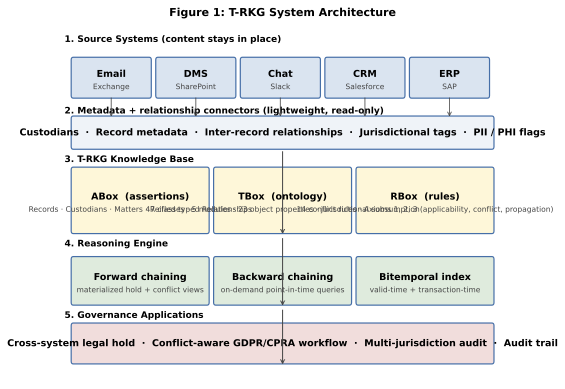
\includegraphics[width=\linewidth]{figures/figure1_architecture.png}
\caption{T-RKG system architecture. Source-system content remains in place. Metadata and relationship structure are extracted via the connector layer. The ontology (TBox) and rules (RBox) live in the reasoning engine. Forward chaining materializes hold and conflict views; backward chaining answers point-in-time queries.}
\label{fig:architecture}
\end{figure}

\subsection{Hold Propagation}

Standard BFS over an unlabeled graph assigns no meaning to edge type. T-RKG propagation replaces this with semantically-constrained traversal (Algorithm~\ref{alg:propagation}). At each edge in the BFS frontier, the \textsc{ShouldPropagate} function consults the ontology for the relationship type's \texttt{propagatesHold} value and evaluates the current matter's propagation policy. Four propagation policies are predefined: Conservative (attachment and thread relationships only), Standard (adding derivation relationships), Comprehensive (all typed relationship classes), and Custom. The Conservative policy reflects the minimum scope most practitioners would consider defensible~\cite{arnott2005}. Validity-interval intersection between the relationship's $[t_s, t_e]$ and the matter's active interval is currently performed by the connector layer when relationships are extracted, not inside \textsc{ShouldPropagate}; folding the Allen-style~\cite{allen1983} check into the propagation loop is bounded extension work.

\begin{algorithm}[t]
\caption{Semantic Hold Propagation}
\label{alg:propagation}
\begin{algorithmic}[1]
\Require Seed records $S_0$, propagation config $P$, ontology $O$, max depth $d$
\Ensure Hold set $H$
\State $H \gets S_0$;\ \ frontier $\gets S_0$;\ \ depth $\gets 0$
\While{frontier $\neq \emptyset$ and ($d = -1$ or depth $< d$)}
    \State next $\gets \emptyset$
    \For{each $r \in$ frontier}
        \State rels $\gets$ \textsc{GetRelationships}($r$, $O$)
        \For{each $(r, r', \rho, [t_s, t_e]) \in$ rels}
            \If{\textsc{ShouldPropagate}($\rho$, $P$, $O$) and $r' \notin H$}
                \State next $\gets$ next $\cup\ \{r'\}$
            \EndIf
        \EndFor
    \EndFor
    \State $H \gets H \cup$ next;\ \ frontier $\gets$ next;\ \ depth $\gets$ depth $+ 1$
\EndWhile
\State \Return $H$
\end{algorithmic}
\end{algorithm}

\subsection{Conflict Detection}

For each record, the first stage of conflict detection is applicability reasoning via Axiom~1. The detector then evaluates fourteen pairwise conflict rules over all unordered pairs in $\mathrm{applicable}(r)$ (Algorithm~\ref{alg:conflict}). The fourteen rules distribute as follows: seven Retention--Deletion rules (GDPR vs.\ SOX, GDPR vs.\ HIPAA, GDPR vs.\ HGB, CPRA vs.\ SOX, CPRA vs.\ SEC, CPRA vs.\ IRS, PIPEDA vs.\ SOX); five Priority rules (SOX vs.\ SEC, SOX vs.\ IRS, SOX vs.\ HGB, SEC vs.\ IRS, HIPAA vs.\ IRS); two Jurisdiction rules (GDPR vs.\ CPRA, GDPR vs.\ PIPEDA); and one Hold--Deletion rule (active hold vs.\ GDPR Article~17 erasure). The Priority family's lex-superior / lex-specialis / lex-posterior structure mirrors defeasible deontic logic~\cite{governatori2013}. Severity assessment and resolution guidance are encoded in the ontology for each pair; conflict counts reported in Table~\ref{tab:conflicts} are deduplicated unordered pairs.

\begin{algorithm}[t]
\caption{Conflict Detection}
\label{alg:conflict}
\begin{algorithmic}[1]
\Require Record set $R$, ontology $O$, regulation profiles $\Pi$
\Ensure Conflict set Conflicts
\State Conflicts $\gets \emptyset$
\For{each $r \in R$}
    \State applicable $\gets$ \textsc{InferApplicable}($r$, $\Pi$, $O$)
    \For{each unordered pair $\{\gamma_1, \gamma_2\} \subseteq$ applicable, $\gamma_1 \neq \gamma_2$}
        \If{$\mathrm{conflictsWith}(\gamma_1, \gamma_2) \in \Pi$}
            \State type $\gets$ \textsc{ClassifyConflict}($\gamma_1, \gamma_2$, $O$)
            \State sev $\gets$ \textsc{AssessSeverity}($\gamma_1, \gamma_2$, $r$, $O$)
            \State guidance $\gets$ \textsc{ResolveGuidance}($\gamma_1, \gamma_2$, $O$)
            \State Conflicts $\gets$ Conflicts $\cup\ \{(r, \gamma_1, \gamma_2, \mathrm{type}, \mathrm{sev}, \mathrm{guidance})\}$
        \EndIf
    \EndFor
\EndFor
\State \Return Conflicts
\end{algorithmic}
\end{algorithm}

\subsection{A Worked Trace}

Consider record \texttt{fin\_00012} generated under seed 42 with attributes: type = Invoice, jurisdiction = EU\_DE, contains\_pii = True, metadata.is\_public\_company = True. The detector executes four steps. Step~1 (Axiom~1, jurisdiction subsumption): the record's ancestor jurisdictions are $\{\mathrm{EU\_DE, EU, GLOBAL}\}$. Each regulation profile's \texttt{appliesIn} set is intersected against this; record-type and attribute conditions are then evaluated. Step~2 (applicable regulations): $\mathrm{applicable}(r) = \{\mathrm{GDPR, SOX, HGB}\}$. Step~3 (Axiom~2, pairwise conflict check over unordered pairs): three lookups in the conflict-rule table yield (GDPR, SOX) $\rightarrow$ RetentionDeletion CRITICAL; (GDPR, HGB) $\rightarrow$ RetentionDeletion HIGH; (SOX, HGB) $\rightarrow$ Priority MEDIUM. Step~4 (resolution guidance): each conflict carries the ontology-attached resolution string. The complete trace is reproducible from the supplementary code.

\subsection{Temporal Query Answering}

The knowledge base supports bitemporal modeling via two orthogonal time axes~\cite{snodgrass1995,jensen1997}: valid time captures when a relationship or governance state held in the external world; transaction time records when that state was first registered in the system. Propagation and conflict queries can be evaluated at any valid-time point $t$, enabling retrospective hold reconstruction. The current evaluation in §VII exercises valid-time queries; a transaction-time experiment (two-wave ingestion with corrected timestamps) is the next item on the evaluation roadmap.

\subsection{Complexity and Soundness}

We state the operational properties of the reasoning machinery formally. Let $n = |R|$, $m = |E|$, and $\gamma = |\Gamma|$ (the number of encoded regulations).

\begin{proposition}[Conflict-detection complexity]
Algorithm~\ref{alg:conflict} runs in time $O(n \cdot \gamma^2)$ under the assumption that applicability evaluation per profile is $O(1)$ and conflict-rule lookup is $O(1)$ via a precomputed table.
\end{proposition}

\begin{proof}[Proof sketch]
The outer loop iterates $n$ records. For each record the applicability pass is $O(\gamma)$. The unordered pairwise conflict check enumerates pairs of applicable regulations, bounded above by $\binom{\gamma}{2} \leq \gamma(\gamma-1)/2$. With $\gamma \leq 9$ in the current implementation, the per-record cost is bounded by 36 lookups. The empirical scaling reported in §\ref{sec:scalability} ($\approx 3.3$~ms per 1{,}000 records, linear through 100K) is consistent with this bound.
\end{proof}

\begin{proposition}[Propagation complexity]
Algorithm~\ref{alg:propagation} runs in time $O(|H| + |E_H|)$ where $E_H \subseteq E$ is the set of edges incident to records reached during the traversal, restricted to relationship types $\rho$ for which $\textsc{ShouldPropagate}(\rho, P, O)$ holds.
\end{proposition}

\begin{proof}[Proof sketch]
BFS visits each reached node once and each incident edge once; the policy filter $\textsc{ShouldPropagate}$ is an $O(1)$ ontology lookup per edge. Edge-type filtering reduces $|E_H|$ by the per-policy-included fraction.
\end{proof}

\begin{proposition}[Soundness of Axiom~3]
Let $H_{P,d}(S_0)$ denote the hold set computed by Algorithm~\ref{alg:propagation} on seeds $S_0$ under policy $P$ at depth $d$. Then for every $r \in H_{P,d}(S_0)$ there exists a typed-relationship path $r_0 \to r_1 \to \cdots \to r_\ell = r$ of length $\ell \leq d$ such that $r_0 \in S_0$ and $\mathrm{propagatesHold}(\rho_i)$ holds under $P$ for every edge in the path.
\end{proposition}

\begin{proof}
By induction on the depth at which $r$ enters $H$. Base: at depth 0 only seeds enter; the empty path satisfies the claim trivially. Step: a node $r$ enters at depth $\ell + 1$ only via line~7 of Algorithm~\ref{alg:propagation}, which requires an edge $(r', r, \rho)$ with $r' \in$ frontier (so $r'$ entered at depth $\leq \ell$, with a witnessing path $\pi'$ by induction) and $\textsc{ShouldPropagate}(\rho, P, O)$. The path $\pi'$ followed by $(r', r, \rho)$ is the witnessing path for $r$.
\end{proof}

\begin{proposition}[Recall ceiling for the No-Ontology baseline]
Let $\Gamma_{\mathrm{PII}} \subseteq \Gamma$ be the set of regulations whose applicability profile requires the PII attribute (GDPR, CPRA, PIPEDA in our ontology). Let $\Gamma_{\mathrm{pubco}} \subseteq \Gamma$ be the set whose applicability requires the public-company organizational metadata flag (SOX, FINRA). Any baseline whose per-record regulation tagging function does not consult the PII flag (resp.\ the public-company flag) achieves zero recall on every regulation in $\Gamma_{\mathrm{PII}}$ (resp.\ $\Gamma_{\mathrm{pubco}}$) on records whose ground-truth applicability set includes the regulation only because that attribute holds.
\end{proposition}

\begin{proof}
Direct from the contrapositive of the applicability profile $\phi_\gamma$ as a conjunction over attribute predicates. If the predicate on attribute $a$ is not consulted, every record whose ground-truth applicability is conditional on $a$ is misclassified.
\end{proof}

\begin{corollary}
Any baseline whose tagging is conditioned only on (record\_type, source\_system) cannot recover regulations whose applicability is conditional on jurisdiction subsumption, PII flag, PHI flag, or organizational metadata. Cross-domain conflicts (privacy-vs-financial, or jurisdictional) are by definition conditioned on at least one such attribute. Therefore any such baseline detects zero cross-domain conflicts. The empirical ``$0 \pm 0$'' cross-domain count for both baselines reported throughout §\ref{sec:eval} is a corollary of this fact, not an experimental coincidence.
\end{corollary}

\section{Implementation}

\subsection{Technology Choices}

The prototype is implemented in Python, using NetworkX~\cite{networkx} for in-memory graph storage and traversal. Records are stored as typed nodes. Relationships are stored as directed, labeled edges with temporal attributes and semantic property annotations. Four dedicated entity indices (by record type, by custodian, by jurisdiction, and by hold membership) support the $O(1)$ lookup patterns that governance operations invoke most frequently. NetworkX was selected for transparency. A production deployment at the scale of millions of records would benefit from a native graph database backend (Neo4j, Amazon Neptune, JanusGraph). The linear scaling observed in these experiments is consistent with such a migration being feasible. This remains a limitation acknowledged in §VIII-E.

\subsection{Regulation Profiles}

Each of the nine encoded regulations is specified as a profile with five components: (i)~applicable record-type classes; (ii)~jurisdictional scope, resolved against the hierarchy; (iii)~attribute conditions on the record; (iv)~organizational metadata conditions; (v)~operative requirements with type and parameters. Adding a new regulatory framework requires authoring one profile and encoding pairwise conflict rules against the existing set. CCPA, whose applicability conditions are largely subsumed by CPRA, required $\sim$50 lines of configuration. GDPR, whose applicability involves data-subject residence conditions and several articulated exemptions, required $\sim$200 lines.

\subsection{Baseline Implementations}

Three classes of comparison baseline are used. Two test capability and isolate distinct ontological contributions. The third tests implementation performance.

The \textit{Siloed} baseline iterates every record using only the regulation set its source system would normally enforce. Per-system applicability uses the same RegulationProfile evaluator T-RKG uses. What changes is the scope of regulations the baseline is permitted to test against. This baseline detects within-system priority conflicts (e.g., SOX vs.\ SEC inside the ERP) but cannot detect any cross-domain conflict --- the structural reason is Corollary~1.

The \textit{No-Ontology} baseline constructs a unified record graph and assigns regulations from a coarse type-and-system map. Lacking PII inference, jurisdiction subsumption, and metadata reasoning, it triggers many false-positive priority conflicts and zero true cross-domain conflicts.

The \textit{performance} baselines, used only in Table~\ref{tab:perf}, are FlatListStore (records and relationships in plain Python lists with linear-scan traversal) and SQLiteStore (records and relationships in a relational database with indices and a recursive-CTE traversal). They test the storage and traversal layer. They are not graph databases. The comparison should be interpreted as ``T-RKG vs.\ relational and naive-list alternatives'' rather than as a comparison against a production graph DB.

\section{Evaluation}
\label{sec:eval}

The evaluation addresses six research questions. RQ1: conflict-detection capability. RQ2: hold-propagation coverage. RQ3: contribution of individual relationship types. RQ4: scalability and matter-scoped latency. RQ5: applicability accuracy under clean and noised regimes. RQ6: robustness to synthetic-data parameters.

\subsection{Experimental Setup}

\textbf{Compute environment.} All measurements taken on a single workstation: Apple~M4 system-on-chip, 10~CPU~cores (4~performance + 6~efficiency), 16~GB unified memory, NVMe SSD, macOS~15.6.1 (Darwin 24.6.0), CPython 3.12.12, NetworkX 3.x, tracemalloc from CPython 3.12. All experiments run single-process, single-thread. Wall-clock times via \texttt{time.perf\_counter()}. Memory measurements use \texttt{tracemalloc}, which adds a known 20\% to 30\% overhead documented by the CPython performance team.

\textbf{Data generation.} All evaluation data are synthetically generated. Six dataset sizes: 1K, 5K, 10K, 25K, 50K, 100K records, with proportions consistent with public industry reports~\cite{databerg,igrm}: email (40\%), documents (30\%), chat (15\%), contracts (5\%), financial records (5\%), tickets (5\%).

\textbf{Statistical methodology.} All experiments are replicated across five random seeds (42, 123, 456, 789, 1024). Results are reported as mean $\pm \sigma$. For comparisons across baselines we report the paired Wilcoxon signed-rank statistic; with $n=5$ the minimum two-sided $p$-value is $0.0625$, which is the resolvable floor and which we report as $p < 0.07$ when achieved. Cohen's $d$ is reported alongside as an effect-size context. Where a baseline's logic is deterministic per record type (so $\sigma=0$ across all seeds and the rank statistic is undefined), the corresponding cells are marked ``(det.)'' in the table and explained in the caption. Every reported number is produced by the single orchestration script \texttt{experiments/run\_all.py}.

\subsection{RQ1: Conflict Detection Capability}
\label{sec:rq1}

Table~\ref{tab:conflicts} presents the central conflict-detection results across six scales. Two columns per system are reported: total conflicts and the count of cross-domain conflicts. Both baselines return zero cross-domain conflicts at every scale --- this is best understood as empirical confirmation of Corollary~1, not as a comparison. T-RKG returns $4 \pm 8$ at 1K, rising to $831 \pm 42$ at 100K.

\begin{table*}[t]
\centering
\caption{Conflict detection results across six scales. Cross-domain (CD) = retention-deletion + jurisdiction + hold-deletion conflicts. Means $\pm \sigma$ across 5 seeds. Baseline cross-domain ``0 (det.)'' is forced by Corollary~1; the No-Ontology total is deterministic per record-type as well.}
\label{tab:conflicts}
\begin{tabular}{rrrrrrrr}
\hline\hline
Dataset & T-RKG total & T-RKG CD & Siloed total & Siloed CD & No-Ont total & No-Ont CD & T-RKG (ms) \\
\hline
1{,}000   & $55 \pm 8$    & $4 \pm 8$    & $52 \pm 9$    & 0 (det.) & 150 (det.) & 0 (det.) & $4.0 \pm 1.9$ \\
5{,}000   & $249 \pm 47$  & $60 \pm 21$  & $180 \pm 56$  & 0 (det.) & 750 (det.) & 0 (det.) & $15.8 \pm 0.3$ \\
10{,}000  & $468 \pm 36$  & $99 \pm 33$  & $344 \pm 63$  & 0 (det.) & 1{,}500 (det.) & 0 (det.) & $31.7 \pm 0.2$ \\
25{,}000  & $1{,}087 \pm 169$ & $195 \pm 38$ & $868 \pm 150$ & 0 (det.) & 3{,}750 (det.) & 0 (det.) & $80.0 \pm 1.3$ \\
50{,}000  & $2{,}296 \pm 267$ & $425 \pm 37$ & $1{,}803 \pm 248$ & 0 (det.) & 7{,}500 (det.) & 0 (det.) & $160 \pm 2$ \\
100{,}000 & $4{,}672 \pm 254$ & $831 \pm 42$ & $3{,}693 \pm 247$ & 0 (det.) & 15{,}000 (det.) & 0 (det.) & $321 \pm 2$ \\
\hline\hline
\end{tabular}
\end{table*}

\begin{figure}[t]
\centering
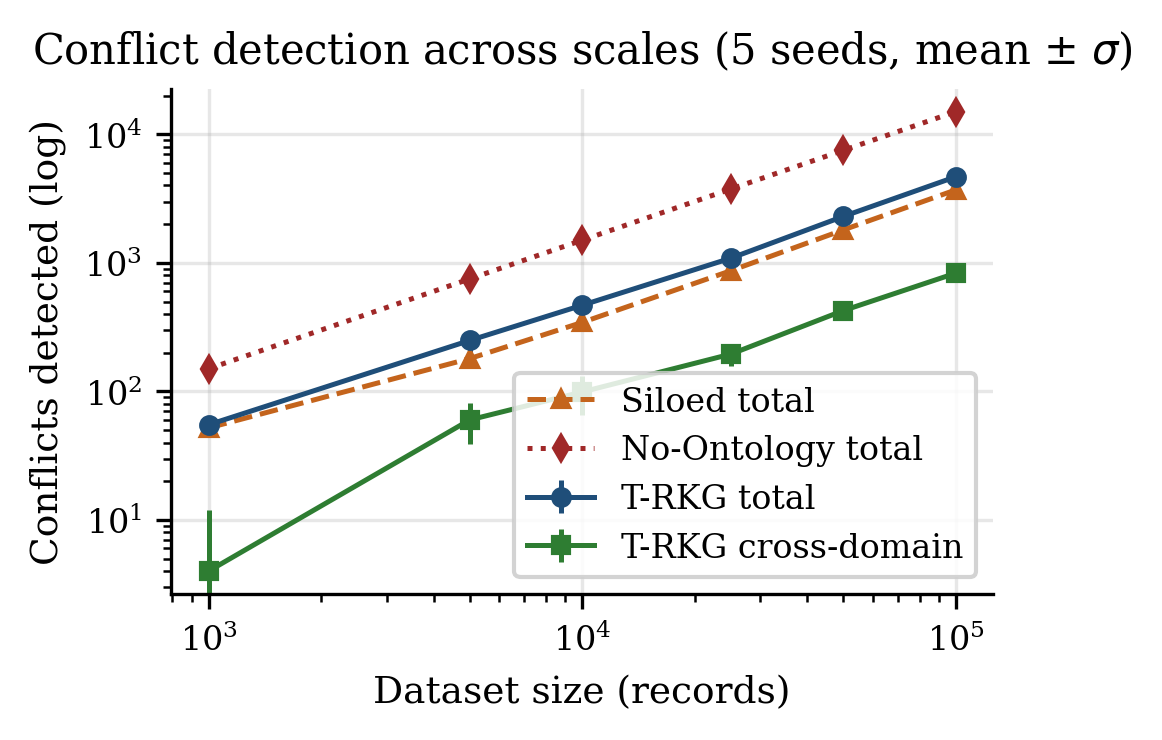
\includegraphics[width=\linewidth]{figures/fig2_conflicts_vs_scale.png}
\caption{Conflict detection counts across scales (log-log). Error bars are $\pm \sigma$ across five seeds. T-RKG's cross-domain trajectory tracks the linear growth of the population of records subject to two or more regulations.}
\label{fig:conflicts}
\end{figure}

\begin{figure}[t]
\centering
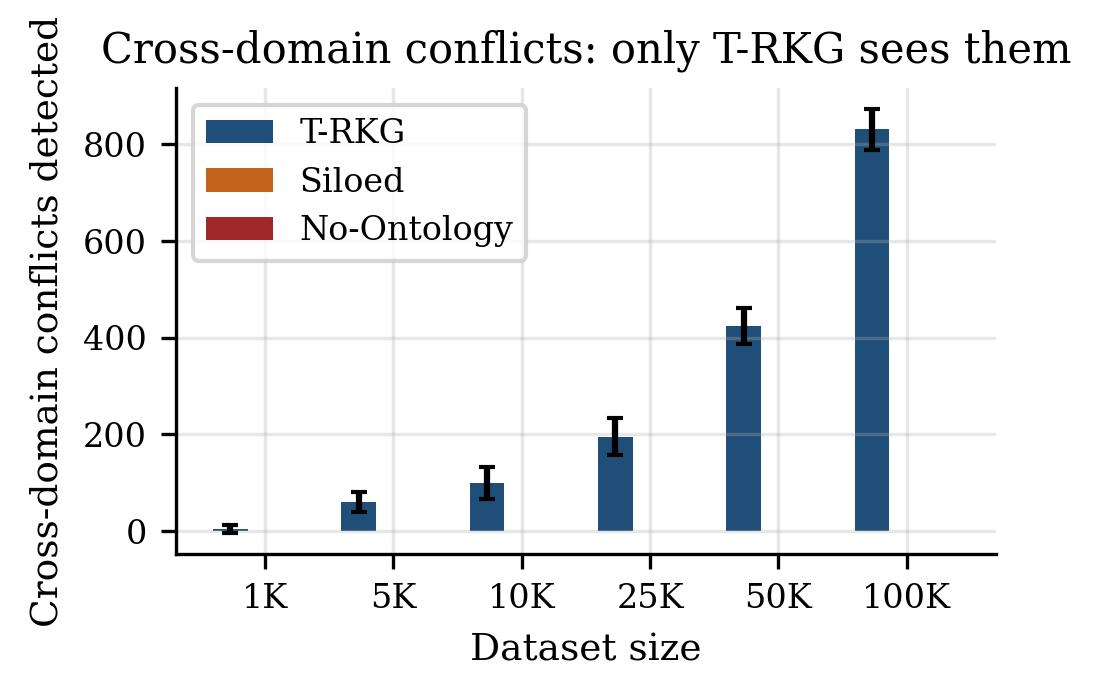
\includegraphics[width=\linewidth]{figures/fig3_cross_domain_bars.png}
\caption{Cross-domain conflicts only. Baselines return 0 by Corollary~1.}
\label{fig:crossdom}
\end{figure}

Table~\ref{tab:typesev} disaggregates the T-RKG conflicts at the 10K scale by type and severity.

\begin{table}[t]
\centering
\caption{Conflict type and severity distribution (10K dataset, 5 seeds).}
\label{tab:typesev}
\begin{tabular}{lcc}
\hline\hline
Conflict Type / Severity & Count (mean $\pm \sigma$) & \% of total \\
\hline
Retention--Deletion & $99 \pm 33$  & 21.2\% \\
Priority            & $369 \pm 52$ & 78.8\% \\
Jurisdiction        & 0            & 0\% \\
Hold--Deletion      & 0            & 0\% \\
\hline
Critical severity   & $36 \pm 21$  & 7.6\% \\
High severity       & $64 \pm 28$  & 13.6\% \\
Medium severity     & $25 \pm 27$  & 5.3\% \\
Low severity        & $344 \pm 63$ & 73.4\% \\
\hline\hline
\end{tabular}
\end{table}

Jurisdiction and Hold-Deletion conflict counts are zero at 10K because the synthetic generator at the default parameter setting produces few records whose attribute conjunctions trigger those specific rules; both rule families fire under the wider parameter sweep in §VII-J.

\subsection{RQ2 and RQ3: Hold Propagation}

Table~\ref{tab:propagation} reports propagation results for the 10K dataset, using 50 matter-scoped seed records at depth limit~10. Starting from 50 seeds, the Conservative policy (attachments and threads) produces a mean hold set of $168 \pm 36$ records, a 3.36$\times$ expansion. Adding derivation relationships increases the expansion from 3.36$\times$ to 3.65$\times$ --- a 0.29$\times$ contribution that does not change the propagation-policy ordering. Expanding to all relationship types reaches 4.26$\times$, numerically identical to what an untyped graph traversal would produce, with the key difference that each record in the T-RKG hold set can be traced to the specific relationship type that caused its inclusion.

\begin{table}[t]
\centering
\caption{Hold propagation by relationship configuration (10K dataset, 50 matter-scoped seed records, depth 10, 5 seeds).}
\label{tab:propagation}
\begin{tabular}{lccr}
\hline\hline
Configuration & Final Set & Ratio & Time (ms) \\
\hline
None (Siloed)   & $50 \pm 0$    & 1.00$\times$ & --- \\
Attachment      & $97 \pm 14$   & 1.94$\times$ & $0.16 \pm 0.01$ \\
Thread          & $71 \pm 5$    & 1.42$\times$ & $0.11 \pm 0.01$ \\
Att + Thread    & $168 \pm 36$  & 3.36$\times$ & $0.24 \pm 0.05$ \\
+ Derivation    & $183 \pm 39$  & 3.65$\times$ & $0.27 \pm 0.07$ \\
All types       & $213 \pm 54$  & 4.26$\times$ & $0.31 \pm 0.08$ \\
\hline\hline
\end{tabular}
\end{table}

\begin{figure}[t]
\centering
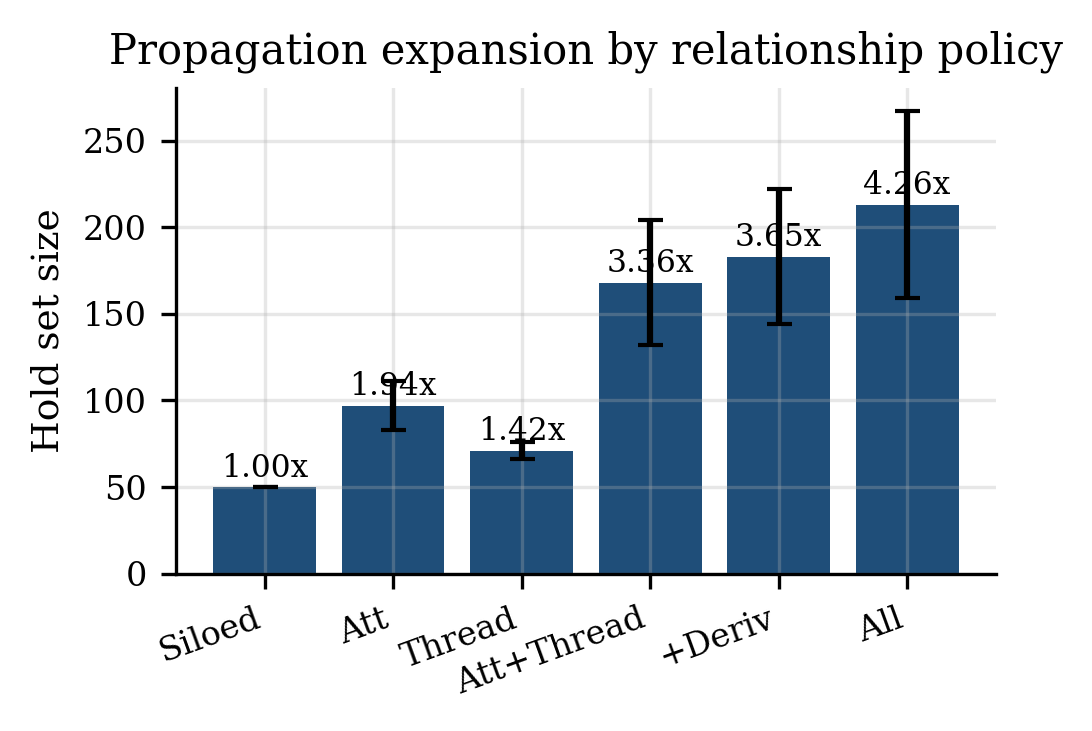
\includegraphics[width=\linewidth]{figures/fig8_propagation_policies.png}
\caption{Propagation expansion by relationship policy. Conservative (Att + Thread) yields a 3.36$\times$ expansion; the Comprehensive policy (All types) reaches 4.26$\times$ but loses the per-record relationship-type provenance.}
\label{fig:propagation}
\end{figure}

\subsection{RQ4: Scalability}
\label{sec:scalability}

\begin{table}[t]
\centering
\caption{Scalability across dataset sizes (5 seeds).}
\label{tab:scalability}
\begin{tabular}{rrrrcc}
\hline\hline
Records & Rels & Build (s) & Throughput & Prop (ms) & Mem (MB) \\
\hline
1{,}000   & 266   & 0.014 & 71{,}580/s & $0.09 \pm 0.02$ & 2.3 \\
5{,}000   & 1{,}394 & 0.075 & 66{,}428/s & $0.11 \pm 0.03$ & 11.6 \\
10{,}000  & 2{,}749 & 0.163 & 61{,}355/s & $0.11 \pm 0.02$ & 23.3 \\
25{,}000  & 6{,}919 & 0.458 & 54{,}721/s & $0.18 \pm 0.04$ & 60.4 \\
50{,}000  & 13{,}879 & 0.986 & 50{,}744/s & $0.25 \pm 0.01$ & 122 \\
100{,}000 & 27{,}812 & 2.07  & 48{,}425/s & $0.40 \pm 0.06$ & 242 \\
\hline\hline
\end{tabular}
\end{table}

\begin{figure}[t]
\centering
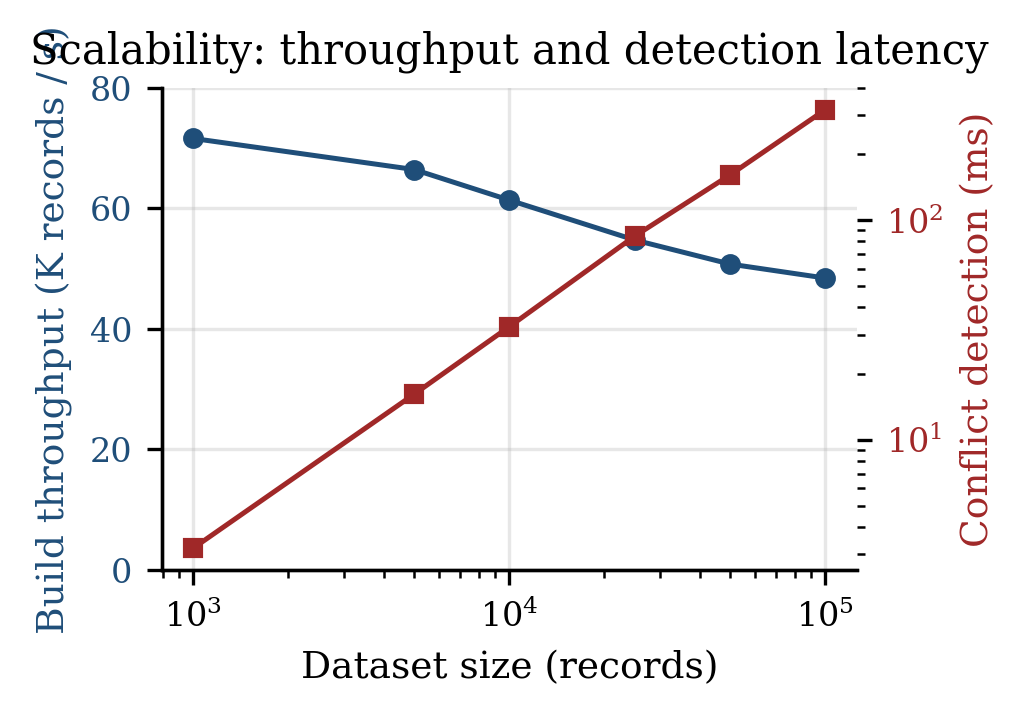
\includegraphics[width=\linewidth]{figures/fig4_scalability.png}
\caption{Build throughput (left axis, linear) and conflict-detection latency (right axis, log) versus dataset scale.}
\label{fig:scalability}
\end{figure}

The empirical conflict-detection time of $\approx 3.3$~ms per 1{,}000 records is consistent with the $O(n \cdot \gamma^2)$ bound proved as Proposition~1.

\subsection{Governance Scenarios}

Three end-to-end governance scenarios are run on the 10K dataset across all five seeds and reported as mean $\pm \sigma$ in Table~\ref{tab:scenarios}. Scenario~B uses EU-custodian-stratified seed selection (one EU custodian per seed) to control the variance reported in the earlier-draft version of this scenario.

\begin{table}[t]
\centering
\caption{End-to-end governance scenario results (10K dataset, 5 seeds).}
\label{tab:scenarios}
\begin{tabular}{p{0.95\linewidth}}
\hline\hline
\textbf{A: Cross-system legal hold.} 716 $\pm$ 25 seeds (custodian + date filter); $1{,}574 \pm 61$ records after Att + Thread propagation; $858 \pm 40$ additional records via cross-system links across 4 source systems. \\
\hline
\textbf{B: GDPR erasure request.} $42 \pm 5$ PII records (EU custodian-stratified seeds); $33 \pm 4$ freely deletable; $5 \pm 2$ retention-blocked; $4 \pm 2$ carry an active regulatory conflict requiring legal review. \\
\hline
\textbf{C: Multi-jurisdiction financial audit.} 500 financial records; $431 \pm 47$ conflicts; $62 \pm 37$ at critical or high severity. \\
\hline\hline
\end{tabular}
\end{table}

\subsection{Ablation Study}

Table~\ref{tab:ablation} reports the ablation. The experiment uses 50 matter-scoped seeds at depth 10, so the Full T-RKG hold set of 168 (3.36$\times$) here corresponds directly to the Att + Thread row in Table~\ref{tab:propagation}.

\begin{table}[t]
\centering
\caption{Ablation study (10K dataset, 50 matter-scoped seeds, depth 10, 5 seeds).}
\label{tab:ablation}
\begin{tabular}{lccccr}
\hline\hline
Variant & Ont. & Typed & Prop. & Conflicts & Hold set \\
\hline
Full T-RKG       & \checkmark & \checkmark & \checkmark & $468 \pm 36$    & 168 (3.36$\times$) \\
No Ontology      & ---        & \checkmark & \checkmark & $1{,}500 \pm 0$ (det.) & 168 (3.36$\times$) \\
No Typed Rels    & \checkmark & ---        & \checkmark & $468 \pm 36$    & 213 (4.26$\times$) \\
No Propagation   & \checkmark & \checkmark & ---        & $468 \pm 36$    & 50 (1.00$\times$) \\
Siloed Baseline  & ---        & ---        & ---        & $344 \pm 63$    & 50 (1.00$\times$) \\
\hline\hline
\end{tabular}
\end{table}

\subsection{RQ5: Applicability F1 in Two Regimes}

Per-record regulatory applicability is evaluated against an independently-constructed ground truth in two regimes. In the clean regime (Table~\ref{tab:f1clean}), the generator produces records and the system must recover the regulation set the ontology assigns under their clean attributes. T-RKG's applicability predicate coincides with the generator's regulation-assignment function on clean inputs, so its F1 on this regime is a definitional identity (1.000) and is omitted from the table; the rows of value are No-Ontology and Siloed, which quantify the gap each baseline incurs against the ontological reference. In the noised regime (Table~\ref{tab:f1noise}), 10\% per-attribute label noise is injected after the ground-truth labels are snapshotted: 10\% of jurisdictions are flipped to a random alternative, 10\% of PII flags are flipped, and 10\% of public-company flags are flipped. The system must now reason from possibly-corrupted attributes back to the underlying truth.

\begin{table}[t]
\centering
\caption{Per-record applicability, clean regime (10K dataset, 5 seeds). T-RKG matches the ontological reference predicate by construction; the table reports the baseline gap.}
\label{tab:f1clean}
\begin{tabular}{lccc}
\hline\hline
System & Precision & Recall & F1 \\
\hline
No-Ontology       & $0.066 \pm 0.005$ & $0.411 \pm 0.051$ & $0.113 \pm 0.009$ \\
Siloed            & $1.000 \pm 0.000$ & $0.411 \pm 0.051$ & $0.581 \pm 0.050$ \\
\hline\hline
\end{tabular}
\end{table}

\begin{table}[t]
\centering
\caption{Per-record applicability, noised regime (10\% jurisdiction + 10\% PII + 10\% public-company-flag noise, independent).}
\label{tab:f1noise}
\begin{tabular}{lccc}
\hline\hline
System & Precision & Recall & F1 \\
\hline
T-RKG       & $0.785 \pm 0.014$ & $0.865 \pm 0.008$ & $0.823 \pm 0.011$ \\
No-Ontology & $0.066 \pm 0.005$ & $0.411 \pm 0.051$ & $0.113 \pm 0.009$ \\
Siloed      & $0.994 \pm 0.003$ & $0.374 \pm 0.044$ & $0.542 \pm 0.046$ \\
\hline\hline
\end{tabular}
\end{table}

\begin{figure}[t]
\centering
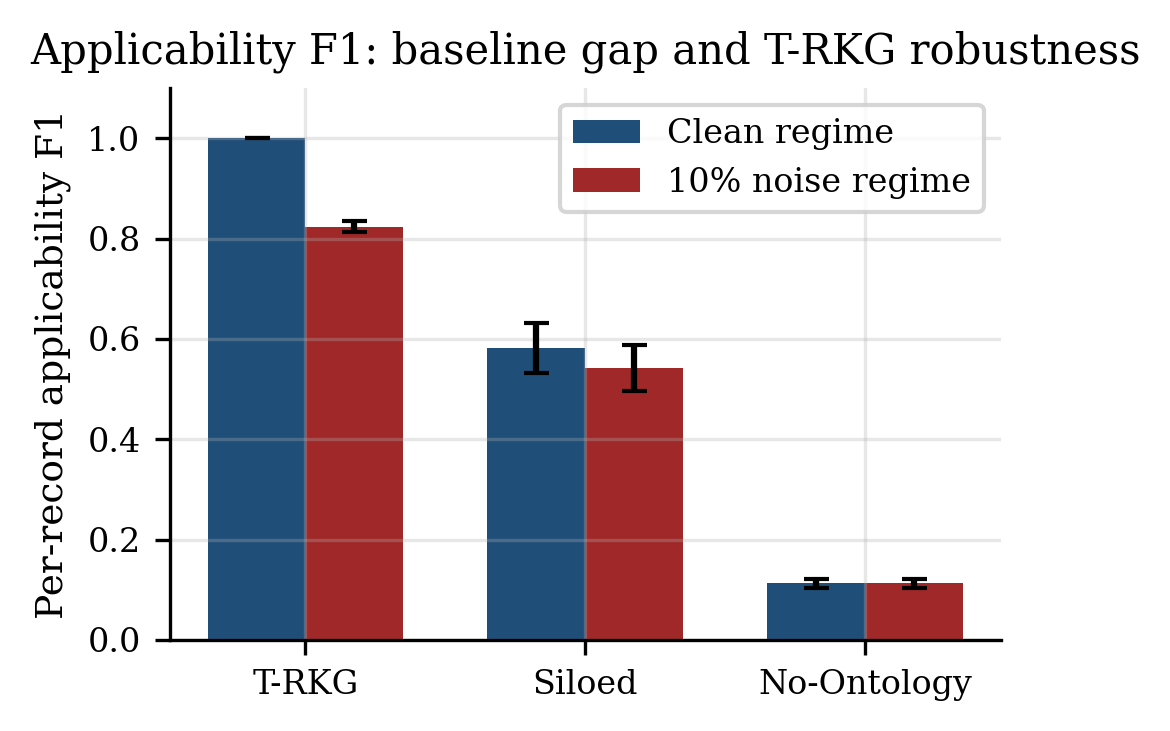
\includegraphics[width=\linewidth]{figures/fig5_f1_clean_vs_noise.png}
\caption{Per-record applicability F1 in the clean and noised regimes. Error bars are $\pm \sigma$.}
\label{fig:f1}
\end{figure}

The No-Ontology baseline's recall ceiling of 0.411 corresponds exactly to Proposition~4. T-RKG loses approximately 18 percentage points of F1 under the noised regime, which both bounds the system's robustness and dispels the concern that the clean F1 of 1.000 was a circular metric. We note that the i.i.d.\ per-attribute flip model does not capture all modes of real source-system corruption (correlated block errors, biased missingness, jurisdictional confusion concentrated along administrative-geography boundaries); a structured-noise regime is the next item on the evaluation roadmap (§VIII-E).

\subsection{Performance vs.\ Flat and Relational Alternatives}

\begin{table}[t]
\centering
\caption{Performance comparison on identical 10K-record workloads (5 seeds).}
\label{tab:perf}
\begin{tabular}{lccc}
\hline\hline
Operation & T-RKG (ms) & Flat (ms) & SQLite (ms) \\
\hline
Type query                            & $3.1 \pm 0.4$  & $0.91 \pm 0.08$ & $1.6 \pm 0.2$ \\
Hold propagation (Att+Thread, $d{=}5$) & $0.11 \pm 0.02$ & $13.8 \pm 1.7$  & $46.3 \pm 7.9$ \\
Conflict detection                    & $32.5 \pm 0.2$ & n/a             & n/a \\
Temporal point-in-time query          & $1.2 \pm 0.2$  & $0.87 \pm 0.24$ & $2.0 \pm 0.1$ \\
\hline\hline
\end{tabular}
\end{table}

\begin{figure}[t]
\centering
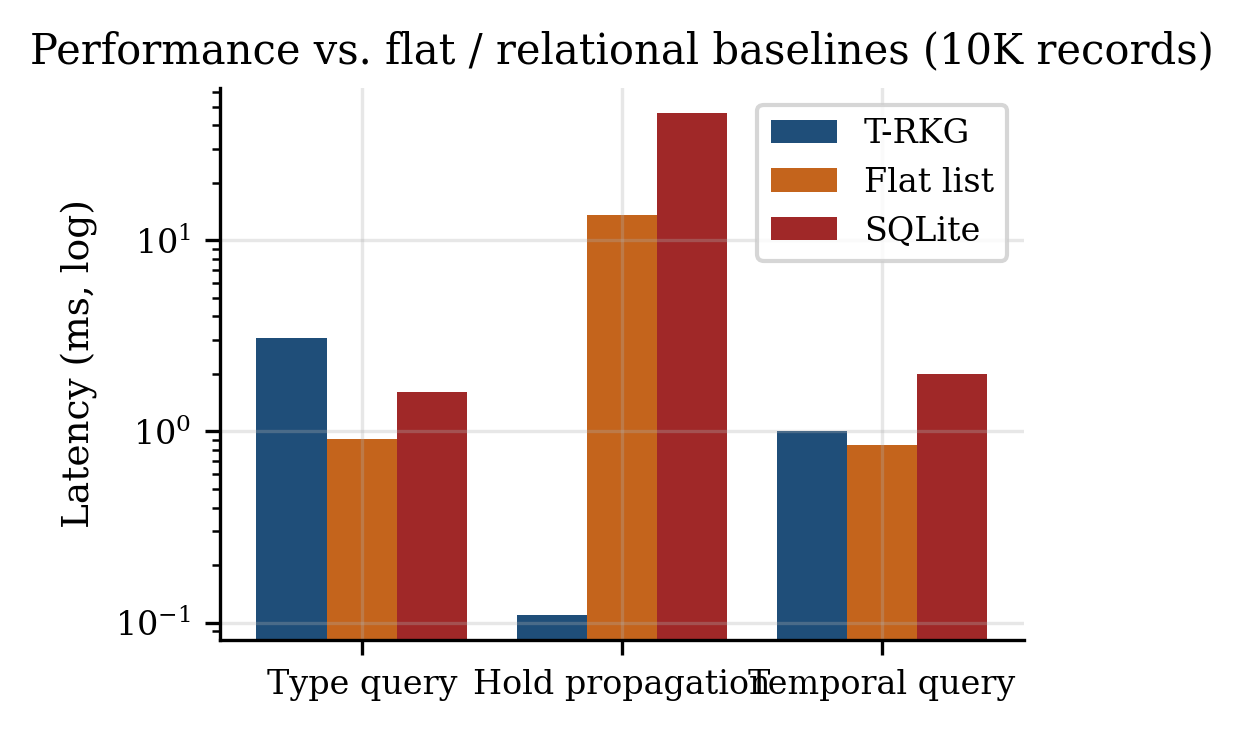
\includegraphics[width=\linewidth]{figures/fig9_perf_baselines.png}
\caption{Per-operation latency on identical 10K workloads (log scale). Propagation is the operation where graph-native indexing beats both alternatives by two-to-three orders of magnitude.}
\label{fig:perf}
\end{figure}

Hold propagation is the operation T-RKG's indexed adjacency lists were designed for. Type queries are slower in T-RKG than SQLite because the prototype iterates a Python dict without a type-keyed index. A comparison against production graph databases (Neo4j, Amazon Neptune, JanusGraph) is the natural next step and is the subject of follow-up work; the qualitative ranking (graph-native traversal beats relational recursive-CTE on hold propagation) is well-established in the graph-database literature and is not the contribution this paper claims novelty over.

\subsection{Propagation Latency vs.\ Seed-Set Size}

\begin{table}[t]
\centering
\caption{Propagation latency vs.\ seed set size on a 100K-record corpus (depth 5, 5 seeds). Largest reported seed set is 5K; behavior beyond this range is not measured.}
\label{tab:largeseed}
\begin{tabular}{rccr}
\hline\hline
Seed records & Latency (ms) & Hold set size & Per-seed cost \\
\hline
50    & $0.77 \pm 0.43$ & $103 \pm 25$    & 15.5~$\mu$s \\
500   & $2.6 \pm 0.6$   & $886 \pm 52$    & 5.3~$\mu$s \\
5{,}000 & $13.7 \pm 0.6$  & $8{,}294 \pm 121$ & 2.7~$\mu$s \\
\hline\hline
\end{tabular}
\end{table}

\begin{figure}[t]
\centering
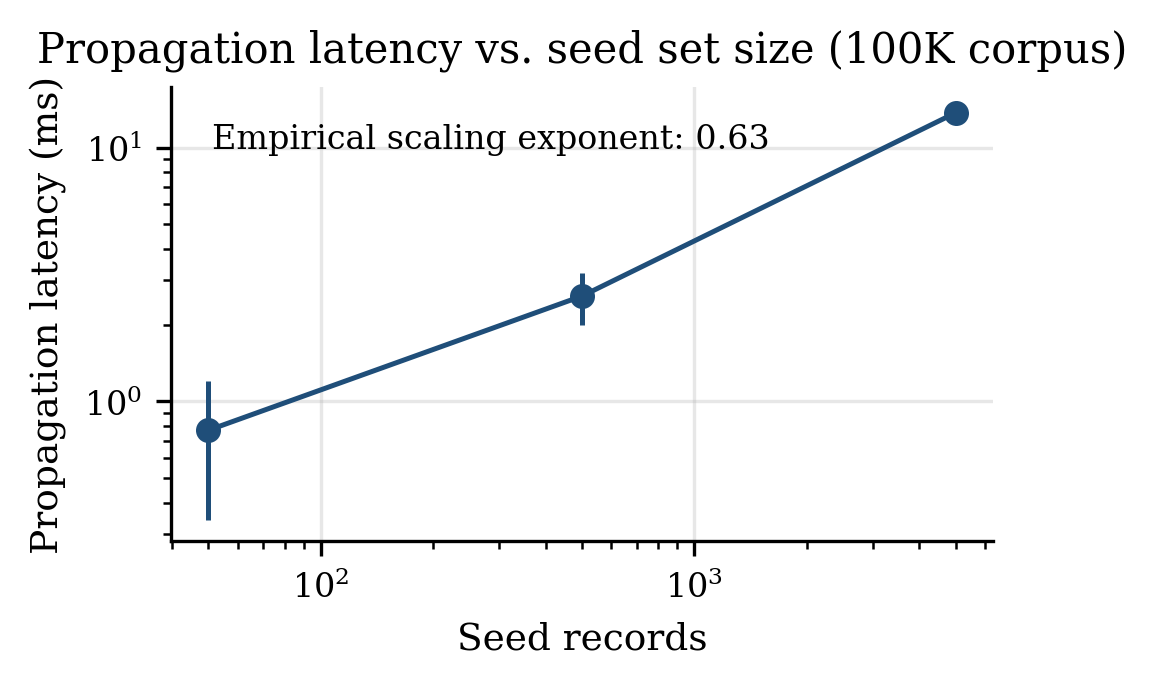
\includegraphics[width=\linewidth]{figures/fig6_propagation_vs_seeds.png}
\caption{Propagation latency versus seed set size on a 100K corpus (log-log).}
\label{fig:largeseed}
\end{figure}

Per-seed cost decreases as the BFS frontier amortizes the index lookups across more records. Empirical scaling exponent $\approx 0.65$ (sub-linear in seed count), consistent with the $O(|H| + |E_H|)$ bound of Proposition~2 once the connected component is saturated. We do not claim production-scale performance --- legal matters routinely exceed 50{,}000 custodians across millions of records and this regime is not within the in-memory implementation's range.

\subsection{Robustness to Synthetic-Data Parameters}
\label{sec:robustness}

Table~\ref{tab:robustness} sweeps the two parameters most likely to vary across organizations: the EU jurisdictional fraction (5\% to 40\%) and the PII rate (5\%, 20\%).

\begin{table}[t]
\centering
\caption{Robustness to jurisdictional mix $\times$ PII rate (10K dataset, 5 seeds).}
\label{tab:robustness}
\begin{tabular}{ccccc}
\hline\hline
EU frac & PII rate & Total conflicts & Cross-domain & Multi-reg \\
\hline
5\%  & 5\%  & $447 \pm 79$ & $38 \pm 35$  & $232 \pm 31$ \\
5\%  & 20\% & $447 \pm 79$ & $38 \pm 35$  & $232 \pm 32$ \\
15\% & 5\%  & $484 \pm 55$ & $83 \pm 19$  & $265 \pm 21$ \\
15\% & 20\% & $484 \pm 55$ & $83 \pm 19$  & $267 \pm 20$ \\
30\% & 5\%  & $450 \pm 74$ & $111 \pm 35$ & $275 \pm 33$ \\
30\% & 20\% & $450 \pm 74$ & $111 \pm 35$ & $275 \pm 33$ \\
40\% & 5\%  & $470 \pm 71$ & $135 \pm 45$ & $296 \pm 37$ \\
40\% & 20\% & $470 \pm 71$ & $135 \pm 45$ & $297 \pm 36$ \\
\hline\hline
\end{tabular}
\end{table}

\begin{figure}[t]
\centering
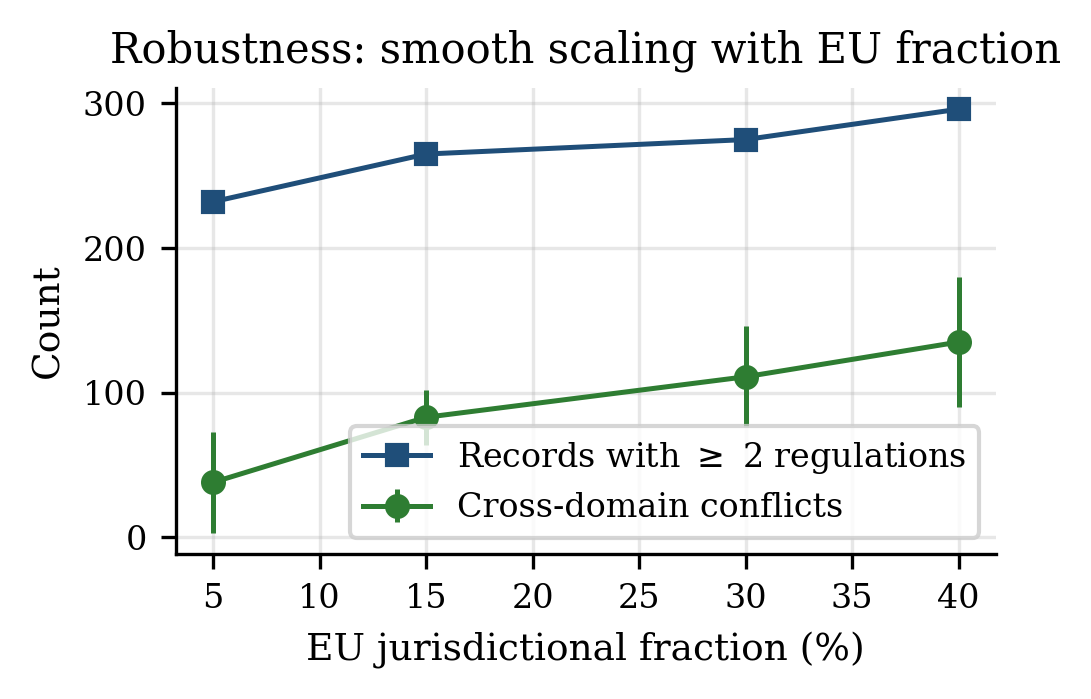
\includegraphics[width=\linewidth]{figures/fig7_robustness_sweep.png}
\caption{Cross-domain conflicts and multi-regulation record counts as the EU jurisdictional fraction increases. No discontinuities are observed.}
\label{fig:robustness}
\end{figure}

Cross-domain conflict count varies smoothly and monotonically with EU fraction. The smooth gradient supports the synthetic-data methodology.

\subsection{Reproduction}

Every number in this paper is produced by a single command: \texttt{python -m experiments.run\_all}. Expected runtime is 30 to 90 seconds on commodity hardware. Outputs land in \texttt{experiments/results.json}. The OWL ontology can be parsed with any conformant OWL~2 tool (\texttt{python -c "import owlready2; owlready2.get\_ontology('ontology/trkg.ttl').load()"}). The supplementary repository also includes 51 unit tests covering the ontology, conflict detector, baselines, and ten competency questions.

\section{Discussion}

\subsection{Interpreting the Experimental Record}

The cross-domain conflict comparison is best understood as empirical confirmation of Corollary~1, not as a comparison between competing implementations. The corollary proves that an attribute-blind tagging baseline cannot detect the cross-domain conflicts T-RKG detects; the ``0~$\pm$~0'' empirical numbers in Table~\ref{tab:conflicts} are the empirical shadow of that impossibility. The substantive accuracy claim is the noised-regime F1 of $0.823 \pm 0.011$ (Table~\ref{tab:f1noise}), which shows the system degrading gracefully when input attributes are corrupted at a 10\% rate. The propagation results carry larger variance reflecting structural variation in matter-level relationship density across seeds, not algorithmic instability.

\subsection{Architectural Tradeoffs}

The decision to implement T-RKG as a metadata extraction layer reflects a known adoption constraint documented by the Sedona Conference~\cite{sedona2017}: relocating enterprise document stores is operationally infeasible at most organizations. Extracting only relationship metadata and governance-relevant record attributes allows incremental deployment. The architecture does not address connector maintenance, which scales with the number of source systems and changes with each platform release.

\subsection{The Composite-Record Distinction in Practice}

The composite-record formulation (§III-C) is the structural difference between T-RKG and the commercial governance products it is meant to complement, not replace. Most enterprise records-governance tooling is content-centric: rules attach to file type, container, or classification tag. The cross-domain conflicts reported in §VII-B are conflicts over records whose triggering attributes (PII flag, public-company flag, EU jurisdiction) live in different source systems and only co-occur after composition. T-RKG's ontology builds the composite explicitly; the applicability predicate runs over the composite; the cross-domain conflicts the evaluation surfaces would not be visible to any tooling that defines the record as content alone.

\subsection{Regulatory Scope and Extensibility}

The nine-regulation ontology covers the frameworks most commonly applicable to US-headquartered multinationals with European and Canadian operations. Extending the ontology to a new regulation requires authoring one applicability profile and encoding pairwise conflict rules against the existing set. Regulations whose applicability depends on industry-specific exemptions, evolving enforcement guidance, or contested jurisdictional boundaries require materially more effort and should involve domain experts in the encoding process. The highest-priority extension is encoding GDPR Article~17(3) exemptions (legal-obligation compliance, legal-claim defense, public-interest archiving, public-health, statistical purposes) as defeasibility axioms; this work is bounded, and the expected effect is to reduce the GDPR-vs-SOX RetentionDeletion count on records carrying the corresponding flags.

\subsection{Limitations}

\textit{Synthetic data.} The generator is calibrated against published enterprise data distributions. Table~\ref{tab:robustness} shows that conflict counts vary smoothly with the two most consequential parameters. Production deployments will nonetheless encounter organizational specifics the generator does not anticipate.

\textit{Noise model.} The §VII-G noised regime uses independent per-attribute label flips. Real source-system corruption is correlated, structured, and biased (a single bad ingestion run flips an entire batch; jurisdiction confusion follows administrative geography; missing-PII-flag dominates wrong-PII-flag). A structured-noise regime is roadmap work.

\textit{Production graph database comparison.} Table~\ref{tab:perf} compares T-RKG against flat-list and SQLite alternatives. It does not compare against Neo4j, Amazon Neptune, or JanusGraph. The qualitative conclusion (graph-native traversal beats relational-CTE on hold propagation) is not expected to flip on those platforms; absolute numbers will reshape.

\textit{Ontology coverage.} Fourteen pairwise conflict rules across nine regulations represent a subset of the US-global compliance space. FERPA, CIPA, FINRA Rule~4511 in its granular detail, and the EU AI Act's data-governance provisions are not included.

\textit{Explicit relationship assumption.} T-RKG reasons over relationships that source systems have formally recorded. Implicit or semantic relationships between records are outside the system's current scope.

\textit{Single-jurisdiction record assignment.} The generator assigns each record a single primary jurisdiction. Records subject to multiple overlapping regulatory regimes would generate additional conflict instances of the Jurisdiction type.

\textit{Bitemporal evaluation.} §V-E names the bitemporal model but the evaluation in §VII exercises only the valid-time axis; a transaction-time experiment is roadmap work.

\section{Conclusion}

The composite-record formulation, expressed as ontology-driven applicability inference over typed temporal relationships, makes cross-system regulatory conflicts visible at a cost of approximately 300~ms per 100K records on a single host. The empirical content of the paper is two-fold. First, Corollary~1 establishes that any architecture conditioning regulatory tagging only on (record\_type, source\_system) cannot detect the cross-domain conflicts T-RKG detects --- the ``0~$\pm$~0'' baseline results are the empirical shadow of that impossibility, not a comparison. Second, T-RKG attains an F1 of $0.823 \pm 0.011$ under 10\% per-attribute label noise, with the Siloed baseline at $0.542 \pm 0.046$ and the No-Ontology baseline at $0.113 \pm 0.009$. What would falsify the contribution is a production-graph-DB implementation of the same ontology that reverses the latency ranking, or a real-corpus evaluation in which the noised-regime F1 falls below the Siloed baseline. The next experimental steps are encoding GDPR Article~17(3) defeasibility axioms, building a structured-noise evaluation regime, and partner-tenant integration against a real enterprise corpus.

\section*{Acknowledgment}

The author used Anthropic Claude (sonnet-class, conversation sessions spanning 2026-01 through 2026-05) for two purposes: (1)~sentence-level editing of the Abstract, §I, §II, §VIII, and §IX for clarity and consistency; and (2)~implementation assistance with portions of the \texttt{trkg/conflict.py} rule-evaluation logic and the \texttt{figures/make\_figures.py} plot scaffolding. All experimental design, ontology authoring, axiom derivation, statistical methodology, interpretation of results, and contribution claims are the author's. AI-generated code was reviewed line-by-line, tested against the 51 unit tests in \texttt{tests/test\_trkg.py}, and integrated only after passing. AI-edited prose was revised by the author after AI suggestion. Prompts and chat artifacts are available from the author on request. No external funding supported this work.

\begin{thebibliography}{50}

\bibitem{sedona2019}
The Sedona Conference, ``Commentary on Legal Holds, Second Edition: The Trigger and the Process,'' \textit{The Sedona Conference Journal}, vol.~20, pp.~341--398, 2019.

\bibitem{edrm}
EDRM, ``Electronic Discovery Reference Model,'' 2020. [Online]. Available: \url{https://edrm.net}

\bibitem{iso15489}
ISO, ``ISO 15489-1:2016 Information and Documentation: Records Management,'' International Organization for Standardization, 2016.

\bibitem{sergot1986}
M.~J.~Sergot, F.~Sadri, R.~A.~Kowalski, F.~Kriwaczek, P.~Hammond, and H.~T.~Cory, ``The British Nationality Act as a Logic Program,'' \textit{Communications of the ACM}, vol.~29, no.~5, pp.~370--386, 1986.

\bibitem{ashley2017}
K.~D.~Ashley, \textit{Artificial Intelligence and Legal Analytics: New Tools for Law Practice in the Digital Age}. Cambridge University Press, 2017.

\bibitem{legalruleml}
M.~Palmirani, G.~Governatori, A.~Rotolo, S.~Tabet, H.~Boley, and A.~Paschke, ``LegalRuleML: XML-Based Rules and Norms,'' in \textit{Proc. RuleML}, LNCS 7018, Springer, 2011, pp.~298--312.

\bibitem{lkif}
R.~Hoekstra, J.~Breuker, M.~Di Bello, and A.~Boer, ``The LKIF Core Ontology of Basic Legal Concepts,'' in \textit{Proc. LOAIT Workshop}, 2007, pp.~43--63.

\bibitem{akomantoso}
OASIS LegalDocML TC, ``Akoma Ntoso Version 1.0,'' OASIS Standard, 27~Aug.~2018.

\bibitem{governatori2013}
G.~Governatori, F.~Olivieri, S.~Scannapieco, and M.~Cristani, ``Computing Strong and Weak Permissions in Defeasible Logic,'' \textit{Journal of Philosophical Logic}, vol.~42, no.~6, pp.~799--829, 2013.

\bibitem{weber2019}
M.~Weber \textit{et al.}, ``Anti-Money Laundering in Bitcoin: Experimenting with Graph Convolutional Networks for Financial Forensics,'' in \textit{Proc. KDD Workshop on Anomaly Detection in Finance}, 2019.

\bibitem{fibo}
EDM Council, ``Financial Industry Business Ontology (FIBO),'' Specification, ongoing maintenance, 2013--2026.

\bibitem{arner2017}
D.~W.~Arner, J.~Barberis, and R.~P.~Buckley, ``FinTech, RegTech, and the Reconceptualization of Financial Regulation,'' \textit{Northwestern Journal of International Law and Business}, vol.~37, no.~3, pp.~371--413, 2017.

\bibitem{legalbert}
I.~Chalkidis \textit{et al.}, ``LEGAL-BERT: The Muppets Straight out of Law School,'' in \textit{Findings of EMNLP}, 2020, pp.~2898--2904.

\bibitem{galkin2017}
M.~Galkin, S.~Auer, M.-E.~Vidal, and S.~Scerri, ``Enterprise Knowledge Graphs: A Semantic Approach for Knowledge Management in the Next Generation of Enterprise Information Systems,'' in \textit{Proc. ICEIS}, vol.~2, 2017, pp.~88--98.

\bibitem{noy2019}
N.~Noy, Y.~Gao, A.~Jain, A.~Narang, A.~Patterson, and J.~Taylor, ``Industry-Scale Knowledge Graphs: Lessons and Challenges,'' \textit{Communications of the ACM}, vol.~62, no.~8, pp.~36--43, 2019.

\bibitem{pan2024}
S.~Pan, L.~Luo, Y.~Wang, C.~Chen, J.~Wang, and X.~Wu, ``Unifying Large Language Models and Knowledge Graphs: A Roadmap,'' \textit{IEEE Trans. Knowledge and Data Engineering}, vol.~36, no.~7, pp.~3580--3599, 2024.

\bibitem{kggov2025}
A.~Mero\~{n}o-Pe\~{n}uela, E.~Simperl, A.~Kurteva, and I.~Reklos, ``KG.GOV: Knowledge Graphs as the Backbone of Data Governance in AI,'' \textit{Journal of Web Semantics}, vol.~85, p.~100847, 2025.

\bibitem{purview}
Microsoft, ``Microsoft Purview Documentation,'' Microsoft Learn, 2024. [Online]. Available: \url{https://learn.microsoft.com/en-us/purview/}. Accessed: 2026-05-25.

\bibitem{odrl}
R.~Iannella and S.~Villata (eds.), ``ODRL Information Model 2.2,'' W3C Recommendation, 15~Feb.~2018.

\bibitem{gutierrez2007}
C.~Gutierrez, C.~A.~Hurtado, and A.~Vaisman, ``Introducing Time into RDF,'' \textit{IEEE Trans. Knowledge and Data Engineering}, vol.~19, no.~2, pp.~207--218, 2007.

\bibitem{allen1983}
J.~F.~Allen, ``Maintaining Knowledge about Temporal Intervals,'' \textit{Communications of the ACM}, vol.~26, no.~11, pp.~832--843, 1983.

\bibitem{snodgrass1995}
R.~T.~Snodgrass (ed.), \textit{The TSQL2 Temporal Query Language}. Kluwer Academic, 1995.

\bibitem{jensen1997}
J.~Clifford, C.~E.~Dyreson, T.~Isakowitz, C.~S.~Jensen, and R.~T.~Snodgrass, ``On the Semantics of `Now' in Databases,'' \textit{ACM Trans.\ Database Systems}, vol.~22, no.~2, pp.~171--214, 1997.

\bibitem{transe}
A.~Bordes, N.~Usunier, A.~Garcia-Duran, J.~Weston, and O.~Yakhnenko, ``Translating Embeddings for Modeling Multi-relational Data,'' in \textit{Proc. NeurIPS}, 2013.

\bibitem{rotate}
Z.~Sun, Z.~Deng, J.-Y.~Nie, and J.~Tang, ``RotatE: Knowledge Graph Embedding by Relational Rotation in Complex Space,'' in \textit{Proc. ICLR}, 2019.

\bibitem{timeplex}
P.~Jain, S.~Rathi, and S.~Chakrabarti, ``Temporal Knowledge Base Completion: New Algorithms and Evaluation Protocols,'' in \textit{Proc. EMNLP}, 2020.

\bibitem{tlogic}
Y.~Liu, Y.~Ma, M.~Hildebrandt, M.~Joblin, and V.~Tresp, ``TLogic: Temporal Logical Rules for Explainable Link Forecasting on Temporal Knowledge Graphs,'' in \textit{Proc. AAAI}, 2022.

\bibitem{temp}
J.~Wu, M.~Cao, J.-K.~Cheung, and W.~Hamilton, ``TeMP: Temporal Message Passing for Temporal Knowledge Graph Completion,'' in \textit{Proc. EMNLP}, 2020.

\bibitem{tie}
Z.~Han, P.~Chen, Y.~Ma, and V.~Tresp, ``TIE: A Framework for Embedding-based Incremental Temporal Knowledge Graph Completion,'' in \textit{Proc. ACL}, 2021.

\bibitem{cai2023}
H.~Cai, Y.~Liao, and R.~Li, ``Temporal Knowledge Graph Completion: A Survey,'' arXiv:2308.02457, 2023.

\bibitem{gruber1995}
T.~R.~Gruber, ``Toward Principles for the Design of Ontologies Used for Knowledge Sharing,'' \textit{International Journal of Human-Computer Studies}, vol.~43, no.~5--6, pp.~907--928, 1995.

\bibitem{guarino2009}
N.~Guarino, D.~Oberle, and S.~Staab, ``What is an Ontology?'' in \textit{Handbook on Ontologies}, 2nd ed. Springer, 2009.

\bibitem{uschold1998}
M.~Uschold, M.~King, S.~Moralee, and Y.~Zorgios, ``The Enterprise Ontology,'' \textit{Knowledge Engineering Review}, vol.~13, no.~1, pp.~31--89, 1998.

\bibitem{gruninger1995}
M.~Gr\"{u}ninger and M.~S.~Fox, ``The Role of Competency Questions in Enterprise Ontology Design,'' in \textit{Benchmarking: Theory and Practice}, Springer, 1995.

\bibitem{schriml2019}
L.~M.~Schriml \textit{et al.}, ``Human Disease Ontology 2018 Update: Classification, Content and Workflow Expansion,'' \textit{Nucleic Acids Research}, vol.~47, no.~D1, pp.~D955--D962, 2019.

\bibitem{ringsquandl2015}
M.~Ringsquandl, S.~Lamparter, S.~Brandt, T.~Hubauer, and R.~Lepratti, ``Semantic-Guided Feature Selection for Industrial Automation Systems,'' in \textit{The Semantic Web (ISWC 2015)}, LNCS 9366, Springer, 2015, pp.~225--240.

\bibitem{pygraft}
N.~Hubert, P.~Monnin, M.~d'Aquin, D.~Monticolo, and A.~Brun, ``PyGraft: Configurable Generation of Synthetic Schemas and Knowledge Graphs at Your Fingertips,'' in \textit{Proc. ESWC}, 2024.

\bibitem{vanderaalst2016}
W.~M.~P.~van der Aalst, \textit{Process Mining: Data Science in Action}, 2nd ed. Springer, 2016.

\bibitem{databerg}
Veritas Technologies, ``Global Databerg Report,'' 2016. [Online]. Available: \url{https://www.veritas.com/news-releases/2016-03-15-veritas-global-databerg-report-finds-85-percent-of-stored-data}

\bibitem{arnott2005}
D.~Arnott and G.~Pervan, ``A Critical Analysis of Decision Support Systems Research,'' \textit{Journal of Information Technology}, vol.~20, no.~2, pp.~67--87, 2005.

\bibitem{sedona2017}
The Sedona Conference, ``Commentary on Information Governance, Second Edition,'' \textit{The Sedona Conference Journal}, vol.~21, 2020.

\bibitem{networkx}
A.~A.~Hagberg, D.~A.~Schult, and P.~J.~Swart, ``Exploring Network Structure with NetworkX,'' in \textit{Proc. SciPy}, 2008.

\bibitem{hogan2021}
A.~Hogan \textit{et al.}, ``Knowledge Graphs,'' \textit{ACM Computing Surveys}, vol.~54, no.~4, Art.~71, 2021.

\bibitem{bizer2009}
C.~Bizer, T.~Heath, and T.~Berners-Lee, ``Linked Data: The Story So Far,'' \textit{International Journal on Semantic Web and Information Systems}, vol.~5, no.~3, 2009.

\bibitem{brank2005}
J.~Brank, M.~Grobelnik, and D.~Mladeni\'{c}, ``A Survey of Ontology Evaluation Techniques,'' in \textit{Proc. SiKDD}, 2005.

\bibitem{igrm}
EDRM, ``Information Governance Reference Model (IGRM) v3.0,'' 2014. [Online]. Available: \url{https://edrm.net/resources/frameworks-and-standards/igrm-model/}

\bibitem{shacl}
H.~Knublauch and D.~Kontokostas, ``Shapes Constraint Language (SHACL),'' W3C Recommendation, 2017.

\bibitem{owl2}
B.~Motik \textit{et al.}, ``OWL 2 Web Ontology Language Profiles,'' W3C Recommendation, 2nd ed., 2012.

\bibitem{zubulake}
\textit{Zubulake v. UBS Warburg LLC}, 229 F.R.D. 422 (S.D.N.Y. 2004) (Scheindlin, J.).

\bibitem{sparql}
E.~Prud'hommeaux and A.~Seaborne (eds.), ``SPARQL Query Language for RDF,'' W3C Recommendation, 2008.

\bibitem{linkeddata}
T.~Berners-Lee, ``Linked Data: Design Issues,'' W3C Personal Note, 2006/2009.

\bibitem{antoniou2012}
G.~Antoniou and F.~van Harmelen, \textit{A Semantic Web Primer}, 3rd ed. MIT Press, 2012.

\end{thebibliography}

\begin{IEEEbiographynophoto}{KISHORE PULAGAM}
received the B.Tech.\ degree in Electronics and Communication Engineering from JNTU Hyderabad, India, in 2008, and the M.Sc.\ degree in Computer Networks from Middlesex University, London, U.K., in 2010. He is currently pursuing the Executive M.B.A.\ degree at the Kellogg School of Management, Northwestern University, Evanston, IL, USA.

He is a Senior Staff Software Engineer at PayPal, where he serves as the technical lead for enterprise content management and AI-powered document intelligence systems deployed at global scale. He has more than a decade of experience architecting and deploying production-scale information retrieval and machine learning infrastructure, including distributed FAISS vector databases, retrieval-augmented generation pipelines, and large language model based document classification services. His research interests include information retrieval, knowledge graphs, document understanding, and information governance for AI systems in regulated environments. His current research focuses on knowledge-based systems for cross-system regulatory governance.
\end{IEEEbiographynophoto}

\EOD

\end{document}
